\section{Theorie}

\begin{align} 
    \intertext{Licht ist eine elektromagnetische Welle, dessen Ausbreitung durch die Maxwell-Gleichungen beschrieben werden kann.
    Die elektrische Feldstärke einer ebenen Welle lässt sich dabei durch}
    \vec{\text{E}} \left(\text{x,t}\right) = \vec{\text{E}}_{0} \, \cos \left(\text{kx} - \omega\text{t} - \delta \right) \label{1}
    \intertext{angeben.
    K steht dabie für die Wellenzahl, $\text{k} = \frac{2\pi}{\lambda}$, mit $\lambda$ für die Wellenlänge, $\omega$ für die Kreisfrequenz und $\delta$ für einen beliebigen Phasenwinkel.
    Für solche Lichtwellen gilt dabei das Prinzip der linearen Superposition, welche besagt, dass an einem Ort P beim eintreffen zweier Lichtwellen eine Überlagerung stattfindet.
    Dadurch das Lichtintensität I einfacher zu beobachten ist als die Feldstärke, und }
    \text{I} = \text{const}\,\lvert\vec{\text{E}}\rvert^{2}\,, \label{2}
    \intertext{folgt sich für die Addition zweier Wellen}
    \text{I}_{\text{ges}} = 2\,\text{const}\,\vec{\text{E}}^{2}_{0}\,\left(1 + \cos (\delta_{2} - \delta_{1})\right). \label{3}
    \intertext{Die Gleichung besteht aus, den Einzelintensitäten, $2\,\text{const}\,\text{E}^{2}_{0}$, sowie dem sogenannten Interferenzterm, dem Cosinusteil, und ist abhängig durch die Phasenlage $(\delta_{2} - \delta_{1})$.
    Die Gesamtintensität kann dabei um $\pm 2\,\text{const}\,\vec{\text{E}}^{2}_{0}$ von dem Mittelwert $2\,\text{const}\,\vec{\text{E}}^{2}_{0}$ abweichen.
    Der Interferenzterm verschwindet, wenn $(\delta_{2} - \delta_{1})$ ein ungerades vielfaches von $\pi$ ist.}
    \intertext{Bei Überlagerung des Lichtes von zwei verschiedenen Lichtquellen wird keine Interferenz beobachtet, da beim zurückkehren angeregter Atome in den Grundzustand Energie in Form von elektromagnetischer Wellen abgegeben wird.
    Diese besitzen eine endliche Länge, welche wiederrum über die Zeit statisch verteilt werden.
    Das führt dazu, dass wenn über einen genügend großen Zeitraum gemittelt wird der Interferenzterm verschwindet, genannt inkohärentes Licht. 
    Kohärentes Licht, ist Licht, welches feste Werte für k, $\omega$ und $\delta$ in der Gleichung (\ref{1}) annimmt für alle emittierten Wellen.
    Ein Beispiel für Kohärentes Licht wäre ein Laser.
    Jedoch kann Interferenz auch mit einer gewöhnlichen Lichtquelle unter geeigneten Bedingungen beobachtet werden.
    Dabei muss das Licht der Lichtquelle in zwei Strahler zerteilt werden, durch einen Strahlenteiler oder eine Doppelblende, wie in Abbildung \ref{Abbildung1}.
    Beide laufen einen unterschiedlich langen Weg und werden wieder im Punkt P zusammengeführt.} \notag
\end{align}

\begin{figure}[H]
    \centering
    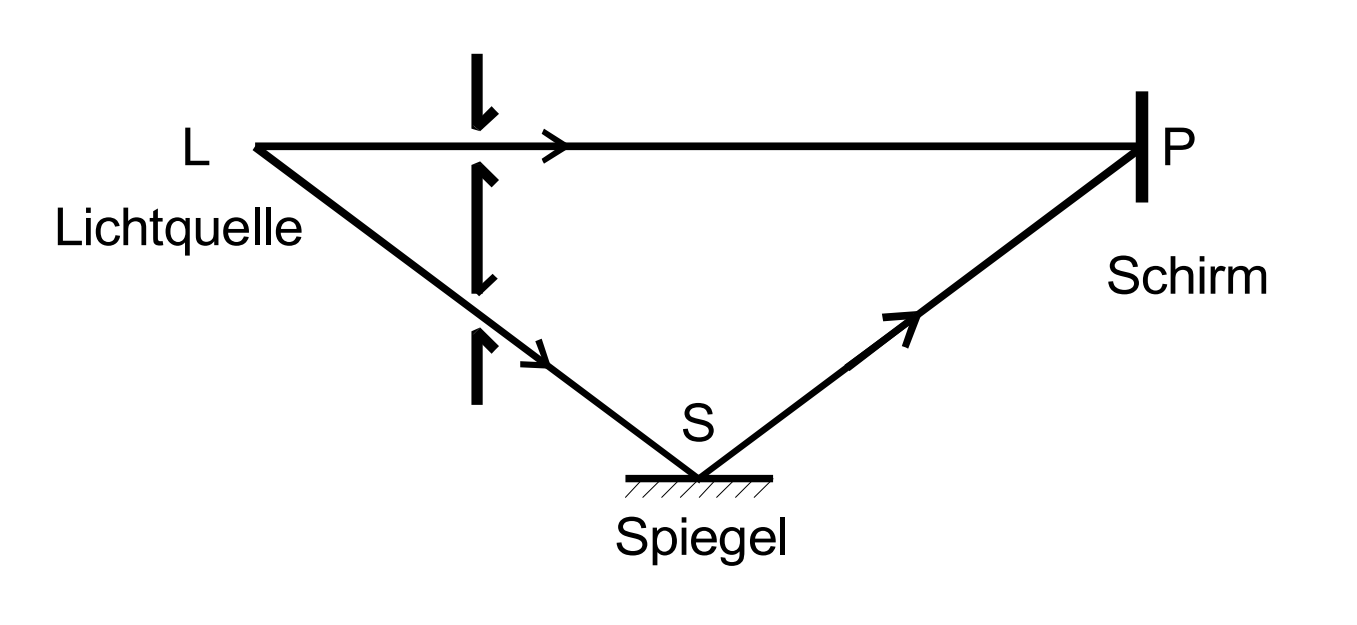
\includegraphics[height=40mm]{bilder/Ab1.png}
    \caption{Prinzipielle Versuchsanordnung zur Erzeugung von Interferenzerscheinungen unter Verwendung
    einer konventionellen Lichtquelle. \cite{a1} \label{Abbildung1}}
\end{figure}

\begin{align}
    \intertext{Die durch den verschiedenen Weg auftretende Phasenverschiebung sorgt wie zuvor für die Interferenz. 
    Es kann jedoch auch dazu kommen, dass keine Interferenz beobachtet werden kann, aufgrund der Kohärenzlänge l. 
    Da der Emissionsakt des Lichtes eine endliche Zeit besitzt, kann diese auch nur eine endliche Länge besitzen.
    Interferenz tritt dabei dann nicht mehr auf, wenn der Wegunterschied der beiden Lichtstrahlen größer ist als die Länge der Lichtzüge, da die Lichtstrahlen zu einem verschiedenen Zeitpunkt am Ort P ankommen.
    Bestimmt kann die Kohärenzlänge l durch die Maximale Anzahl an beobachtbaren Interferenzmaxima N im Punkt P multipliziert mit der Wellenlänge $\lambda$ }
    \text{l} = \text{N}\cdot\lambda \,. \label{4}
\end{align}

\subsection{Das Michelson-Interferometer}

\begin{flushleft}
    Bei dem Michelson-Interferometer wird ein Lichtstrahl, durch das in der Mitte befindende semipermeable Material, geteilt.
    In der Abbildung \ref{Abbildung2} ist der Aufbau dieser Apparatur veranschaulicht.
\end{flushleft}

\begin{figure}[H]
    \centering
    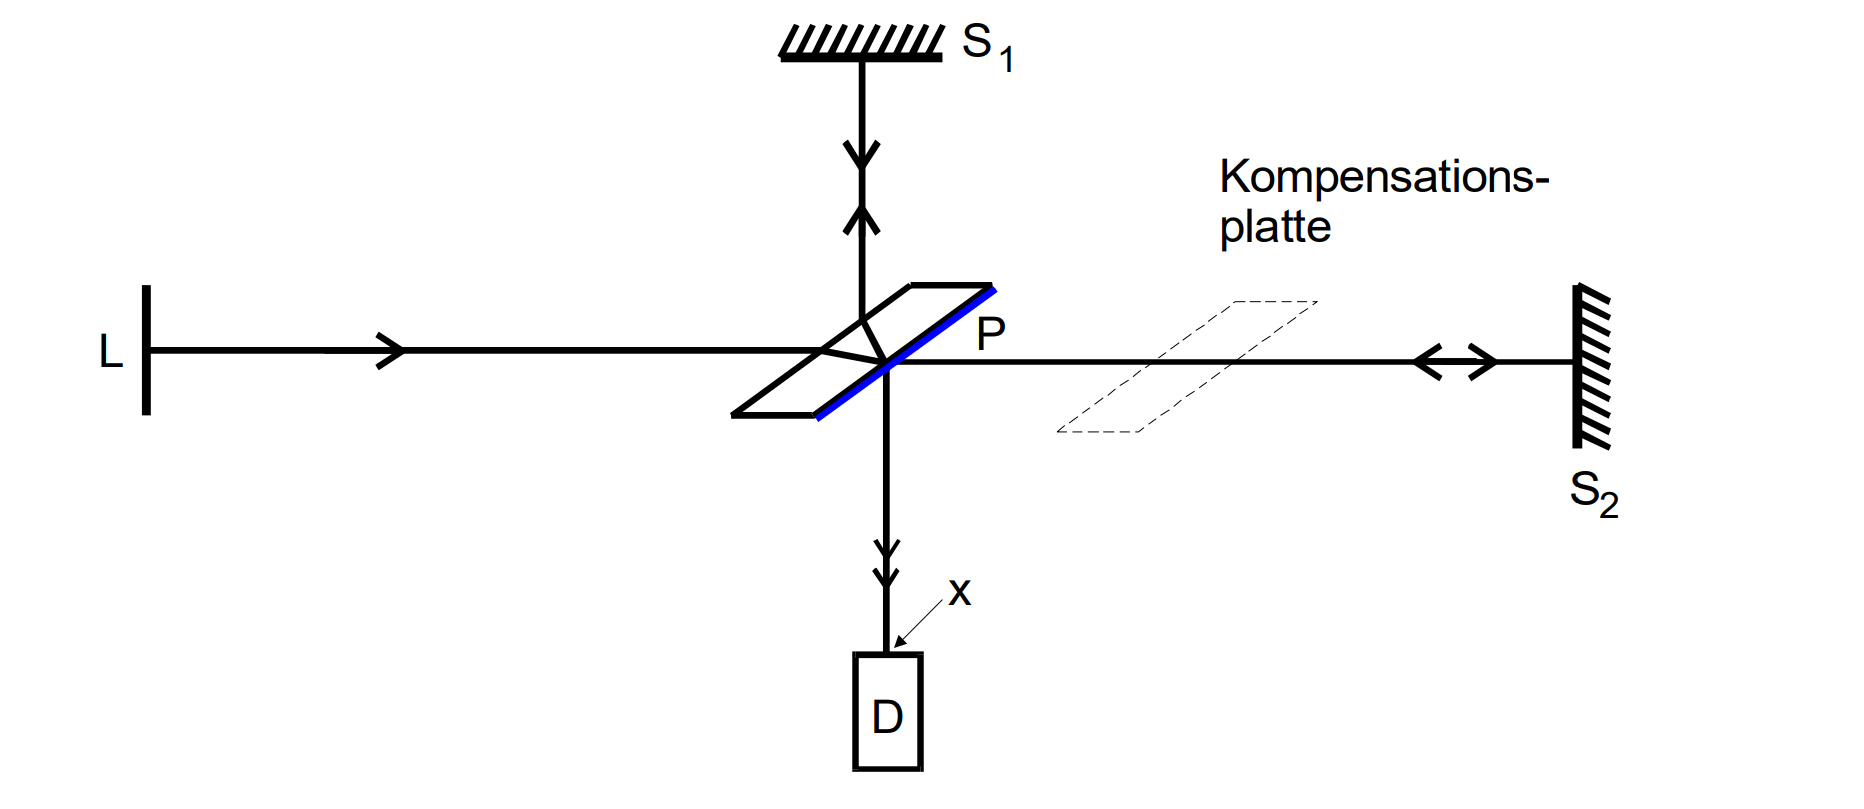
\includegraphics[height=53mm]{bilder/Ab2.png}
    \caption{Prinzipieller Aufbau eines Michelson-Interferometers (L = Lichtquelle, S1 und S2 Spiegel, P = semipermeabler Spiegel, D = Lichtdetektor) \cite{a1}. \label{Abbildung2} }
\end{figure}

\begin{align}
    \intertext{Einer der beiden geteilten Strahlen geht dabei durch das semipermeable Material und trifft auf den Spiegel $\text{S}_{2}$ und der andere wird an der Platte P zum Spiegel $\text{S}_{1}$ reflektiert. 
    An beiden Spiegeln werden die Lichtstrahlen wieder zur Platte P reflektiert, wo die Lichtstrahlen sich wieder teilen.
    Betrachtet werden von den Lichtstrahlen nur die, die parallel zum Detektor laufen.
    Da die Kohärenz der beiden Strahlen wichtig für die Interferenz ist, müssen beide Strahlen kohärent sein.
    Daher sind die Wege $\overline{\text{S}_{1}\,\text{P}}$ und $\overline{\text{S}_{2}\,\text{P}}$ nahezu identisch, jedoch liegt aud dem Weg von P zu $\text{S}_{2}$ eine Kompensationsplatte.
    Diese ist für den Ausgleich der optischen Weglänge des Strahles zuständig, da der Lichtstrahl von $\text{S}_{1}$ zum Punkt P dreimal so oft durchläuft, wie $\text{S}_{2}$ zum Punkt P.
    Bei genau gleichen Längen von den Spiegeln zu dem Punkt P wird ein Gangunterschied D von $\frac{\lambda}{2}$ vorhanden, wobei sich die Lichtstrahlen dort auslöschen. 
    Verändern kann man die Intensität des Interferenzmusters am Ort D durch das Verschieben um $\increment \text{d}$ eines Spiegels}
    \increment \text{d} = \text{z} \cdot \frac{\lambda}{2}\,. \label{5}
    \intertext{Durch diesen Zusammenhang kann die Wellenlänge der verwendeten Lichtquelle bestimmt werden, dabei ist z die Anzahl der beobachteten Interferenzmaxima. 
    Eine weiterer Weg um den optischen Wegunterschied zu erzeugen ist, wenn beide Lichtstrahlen durch ein Medium der Länge b mit einem anderen Brechungsindex laufen.
    Zusehen ist dies in Abbildung \ref{Abbildung3} mit dem Brechungsindex $\text{n} + \increment\text{n}$.  } \notag
\end{align}

\begin{figure}[H]
    \centering
    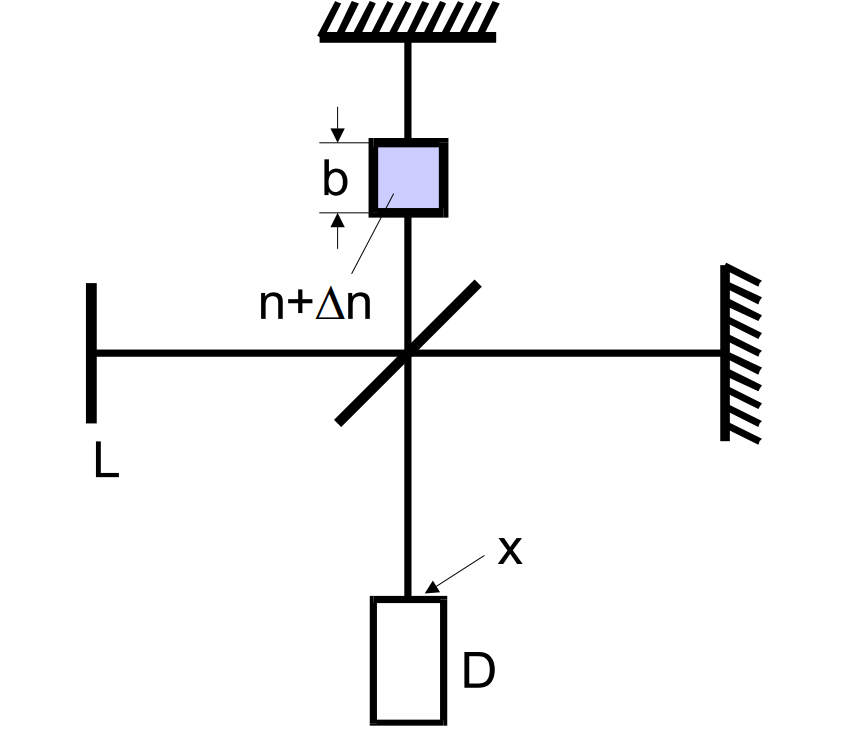
\includegraphics[height=53mm]{bilder/Ab3.png}
    \caption{ Prinzipielle Versuchsordnung zur Messung kleiner Brechungsindexunterschiede mit dem
    Michelson-Interferometer \cite{a1}. \label{Abbildung3} }
\end{figure}

\begin{align}
    \intertext{Der Wegunterschied der beiden Lichtstrahlen beträgt $\increment \text{n}\,\text{b}$. 
    Bei Evakuierung von der Messzelle vergrößert sich der Wegunterschied, sind z Interferenzen am Ort D beobachtbar.
    Über die Formel}
    \text{b} \cdot \increment \text{n} = \frac{\text{z}\,\lambda}{2}\,. \label{6}
    \intertext{Es lässt sich zeigen das die Formel}
    \text{n} = \sqrt{1 + \text{f}(\lambda) \, \text{N}}\,, \notag
    \intertext{gilt. 
    N steht dabei für die Anzahl von Molekülen die zu Schwingung, durch Lichtwellen, angeregt werden.
    Näherungsweise kann die Formel für Licht im sichtbaren Bereich zu}
    \text{n} = 1 + \frac{\text{f}}{2}\,\text{N}\,, \notag
    \intertext{umgrformt werden.} \notag
\end{align}

\begin{align}
    \intertext{Als Vorraussetzung eird angenommen, dass die benutzten Gase Ideale Gase sind.
    Deswegen werden die Anzahl der Moleküle bei Druck p mit Temperatur T gegeben durch}
    \text{N}(\text{p, T}) = \frac{\text{p} \,\, \text{T}_{0}}{\text{T} \,\, \text{p}_{0}}\,\text{N}_{\text{L}}\,.     \\
    \intertext{ $\text{N}_{\text{L}}$ steht dabei für die Loschmidtsche Zahl, $\text{p}_{0}$ der Normaldruck und $\text{T}_{0}$ die Normaltemperatur. 
    Für den Brechungsindex ergibt sich dadurch}
    \increment \text{n}(\text{p, p´}) = \frac{\text{f}}{2}\,\text{N}_{\text{L}}\,\frac{\text{T}_{0}}{\text{p}_{0}}\,\frac{1}{\text{T}}\, \left(\text{p} - \text{p´}\right)\,.     \\
    \intertext{Für den Brechungsindex mit den Normalbedingungen gilt}
    \text{n}(\text{p}_{0}, \text{T}_{0}) = 1 + \increment \text{n}(\text{p, p´})\,\frac{\text{T}}{\text{T}_{\text{0}}}\,\frac{\text{p}_{\text{0}}}{\text{p} - \text{p´}}\,.
    \intertext{Durch einsetzen der Gleichung (\ref{4}) für $\increment \text{n}$ folgt die endgültige Gleichung }
    \text{n}(\text{p}_{0}, \text{T}_{0}) = 1 + \frac{\text{z}\lambda}{2\text{b}}   \,\frac{\text{T}}{\text{T}_{\text{0}}}\,\frac{\text{p}_{\text{0}}}{\text{p} - \text{p´}}\,. \label{10}
\end{align}
